\section{Overview}
The system we present here aims to be easy to use for users, and easy to deploy for venue owners and event organizers. At the same time, it follows the design principles of decentralized contact tracing:

\begin{itemize}
\item Privacy by design: no private/sensitive data should be stored in any central database. Moreover, private data should not be derivable from data (e.g., logs) that are stored for operational purposes.
\item Purpose limitation by design: abusing the system for population control, location tracing, or other objectives other than sending notifications should be difficult if not impossible.
\item Voluntary basis: Use of the digital system is not mandatory. A non-digital fallback must always be available.
\end{itemize}

The system design makes the following assumptions:

\begin{enumerate}
\item The digital system requires the use of an app on the user’s device\footnote{This app can be either separate or integrated with existing proximity tracing solutions. In either case, the system must be designed such that the privacy properties of both proximity and presence tracing  are guaranteed. (This is the case for the design proposed later on in this document.)}
\item Presence tracing should be possible even if the SARS-CoV-2-positive person did not themselves use the app.
\item Users can be trusted to follow notifications from the app, just like they would when notified by a digital contact tracing app.
\end{enumerate}

The first assumption guarantees that the system can notify all visitors, even if the SARS-CoV-2-positive person did not themselves use the app. The second assumption is in line with the current classic approach, which assumes that visitors put their actual phone numbers and name in the attendance logs (there is empirical evidence that many fake numbers are used). In fact, one can reasonably expect better compliance from a privacy-preserving digital solution (where citizens should take action when actually exposed) vs. the classic solutions (where citizens should take action (i.e, write down their real phone number) when attending the venue).

\subsection{A walkthrough of the system}
The following example illustrates how the CrowdNotifier system would work. For illustration, we use a venue as location (e.g., an association’s meeting place, a mosque, a church, a meeting room, a bar, a restaurant, a night club), but we recall that a location could also represent an event that spans different locations (e.g., a demonstration). 

\paragraph{Setting up}
Figure~\ref{fig:overview} gives an overview of the proposed digital system. Suppose Charlie manages a venue. To comply with the regulations, she decides to use the system. To do so, she first uses the system to generate and print two QR codes: an entry code and a tracing code. She posts the entry code at the entrance of the room, and keeps the tracing code private. See Figure O, Setup.

\paragraph{Attending the event/venue}
Attendees have a choice to use their app or not. If they do not, they, for instance, write their name and phone number on an attendee list. If they do, they use their app to scan the QR code posted at the entry to the venue. The app shows the name of the venue as a confirmation. See Figure~\ref{fig:overview}, Entering a venue/event.

Optionally, the user scans another QR code upon leaving the venue to record the departure time.

Their phone will store a private record including the time and location visited. (It does not store the name.) Neither the user, nor anyone with access to the user’s phone, can use the stored records to determine which location the user visited.

\begin{figure}
  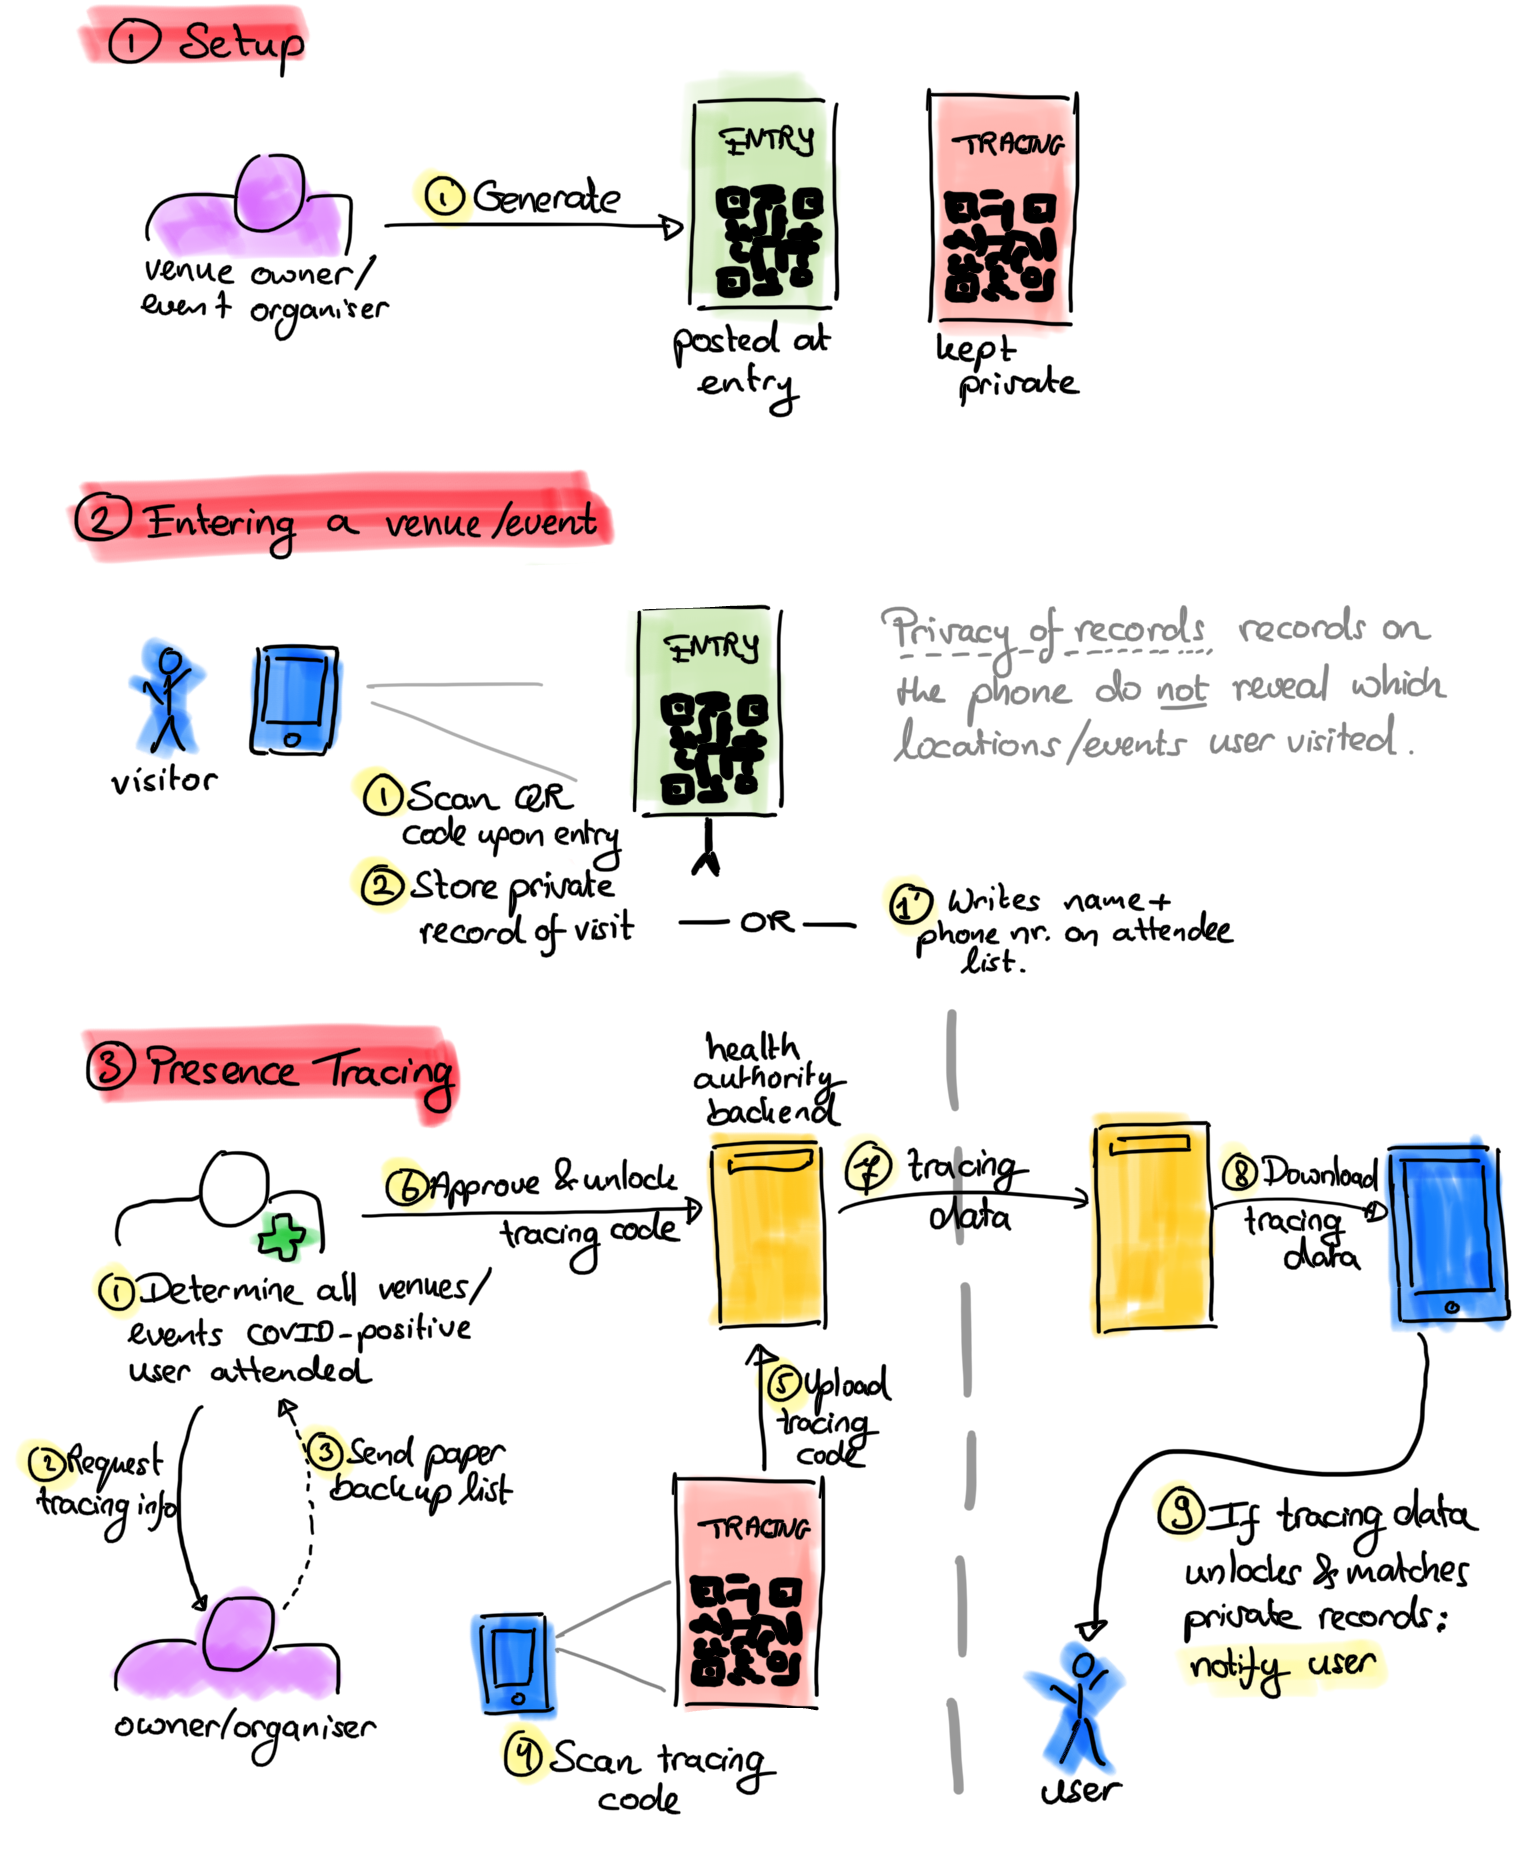
\includegraphics[width=\textwidth]{figures/overview}
  \caption{\label{fig:overview}Overview of the core operations in our proposal for Presence Tracing}
\end{figure}

\paragraph{Presence tracing}
Health officials use the traditional interviewing process to determine which events / locations the SARS-CoV-2-positive person attended (step 1). The health official then contacts the owner/organiser for each of these, requesting two things (step 2):

\begin{enumerate}
\item The paper backup list (step 3)
\item That the owner/organiser uploads the tracing QR code (steps 4 and 5)
\end{enumerate}

Finally, the health official checks and approves the uploaded tracing data (step 6). This ensures that the data corresponds to the requested venues.

The health authority’s backend then disseminates the tracing data (step 7 and 8) to all users of the system. Phones use the provided tracing data to try and unlock private records stored on the phone. If unlocking succeeds, it means that the user was at a location with a SARS-CoV-2-positive person. The phone then determines if there is an epidemiologically relevant overlap between the user’s time at the location and that of the SARS-CoV-2-positive person. If there is, the phone notifies the user (step 9).
